\section{Echo State Networks}
\label{CH:ESN}

Neural networks mimic the human brain in its information processing and can be distinguished into two classes: feedforward neural networks (FFNs) and recurrent neural networks (RNNs). As the names suggest, the feedforward neural networks process information in a sequential structure. They may consist of multiple layers who enable complex nonlinear calculations. Recurrent neural networks may contain cyclical paths and are able to remember past information. When the input has an autoregressive structure, the RNN can remember past information and is much more performant than a feedforward neural network. However, the optimization of these networks is computationally expensive and can become numerically critical. Gradients can vanish or the optimization can become stuck in local minima which makes the optimization of networks inefficient \citep{Bengio1994}.

Echo State Networks naturally tackle the problem of vanishing gradients or local minima. They have the structure of a recurrent neural network, but are much larger and the internal connections of the neural network remain fixed during the training which reflects the concept of reservoir computing.

\cite{Grigortega2018Univeral} show the universality of Echo State Networks for discrete-time fading memory filters with uniformly bounded inputs. \cite{Ortega2018UniversalityStochInput} extend the universality to stochastic semi-infinite inputs\footnote{Universality is referring to arbitrary close approximation of functionals in $L^p(\Omega, \mathcal{F}, \mathbb{P})$ on a probability space $\Omega$ with filtration $\mathcal{F}$ and probability measure $\mathbb{P}$.}.

In the following, we want to focus on the Echo State Network which is desirable because of its simplicity and fast training. It is also the model that has been worked with the most.

\subsection{Architecture}
\label{CH:ESN:Architecture}

An Echo State Network, as mentioned earlier, resembles a recurrent neural network, especially in its architecture. It is also sometimes referred to as an extension of recurrent neural networks, but this is difficult so say. Basically, it only is a different approach to the training and usage of recurrent neural networks, keeping most of the network untrained. Let $K \in \N$ be the number of inputs, $N \in \N$ be the number of neurons and $L \in \N$ be the number of outputs. Let $\bx_t = \left(x_1^t, ..., x_N^t\right) \in \R^{N}$ be the row vector of network activations at time $t \in \Z$ and $f: \R \to \R$ be an elementwise applied activation function. All connections within the system will be denoted by matrices. We will denote by $\win \in \R^{N\times K}$ the connections from the input to the reservoir, by $W \in \R^{N\times N}$ we will denote the internal connections and $\wout \in \R^{L \times N}$ will represent the hidden-to-output connections. The network will also be equipped with a bias $\bb = b\cdot \wbias \in \R^{N}$.
Let $(u_t)_{t\in\Z}$ be an input signal which is discretized in time. Then, the evolution of the network - producing an output value $y_t$ - can be characterized as follows:
\begin{eqnarray}
    \bx_{t} & = & f\left(W\bx_{t-1} + \win u_t +  \bb\right) \label{EQ:ReservoirUpdate} \\
    y_t & = & \bx_{t} \wout \label{EQ:ReservoirReadout}
\end{eqnarray}
where the bias $\bb = b \cdot \wbias$ for a fixed and random matrix $\wbias \in \R^{N}$ and $b \in \R$.
Usually, \refp{EQ:ReservoirReadout} is presented as $y_t = h(\bx_t)$ for any map $h: \R^n \to \R$ but we will focus on the linear case. The readout $h$ can also incorporate the input but for the ease of notation we will work with none of the two. The expression $\wout$ is to be seen as $\bbeta$ from section \ref{CH:LinearRegression}.
The convincing argument of Echo State Networks, which also translates to other reservoir computing models, is the fact that all of its architecture except for $\wout$ is left untrained and doesn't require any training. The \textit{training} of the hidden-to-output connections, by choice of $h$ as linear function, finally boils down to the estimation of a linear regression from section \ref{CH:LinearRegression}, where $\wout$ is now referring to the parameter vector $\bbeta$ from that section.
Figure \refp{FIG:ESNArchitecture} presents the basic ESN architecture.

\begin{figure}
    \begin{center}
    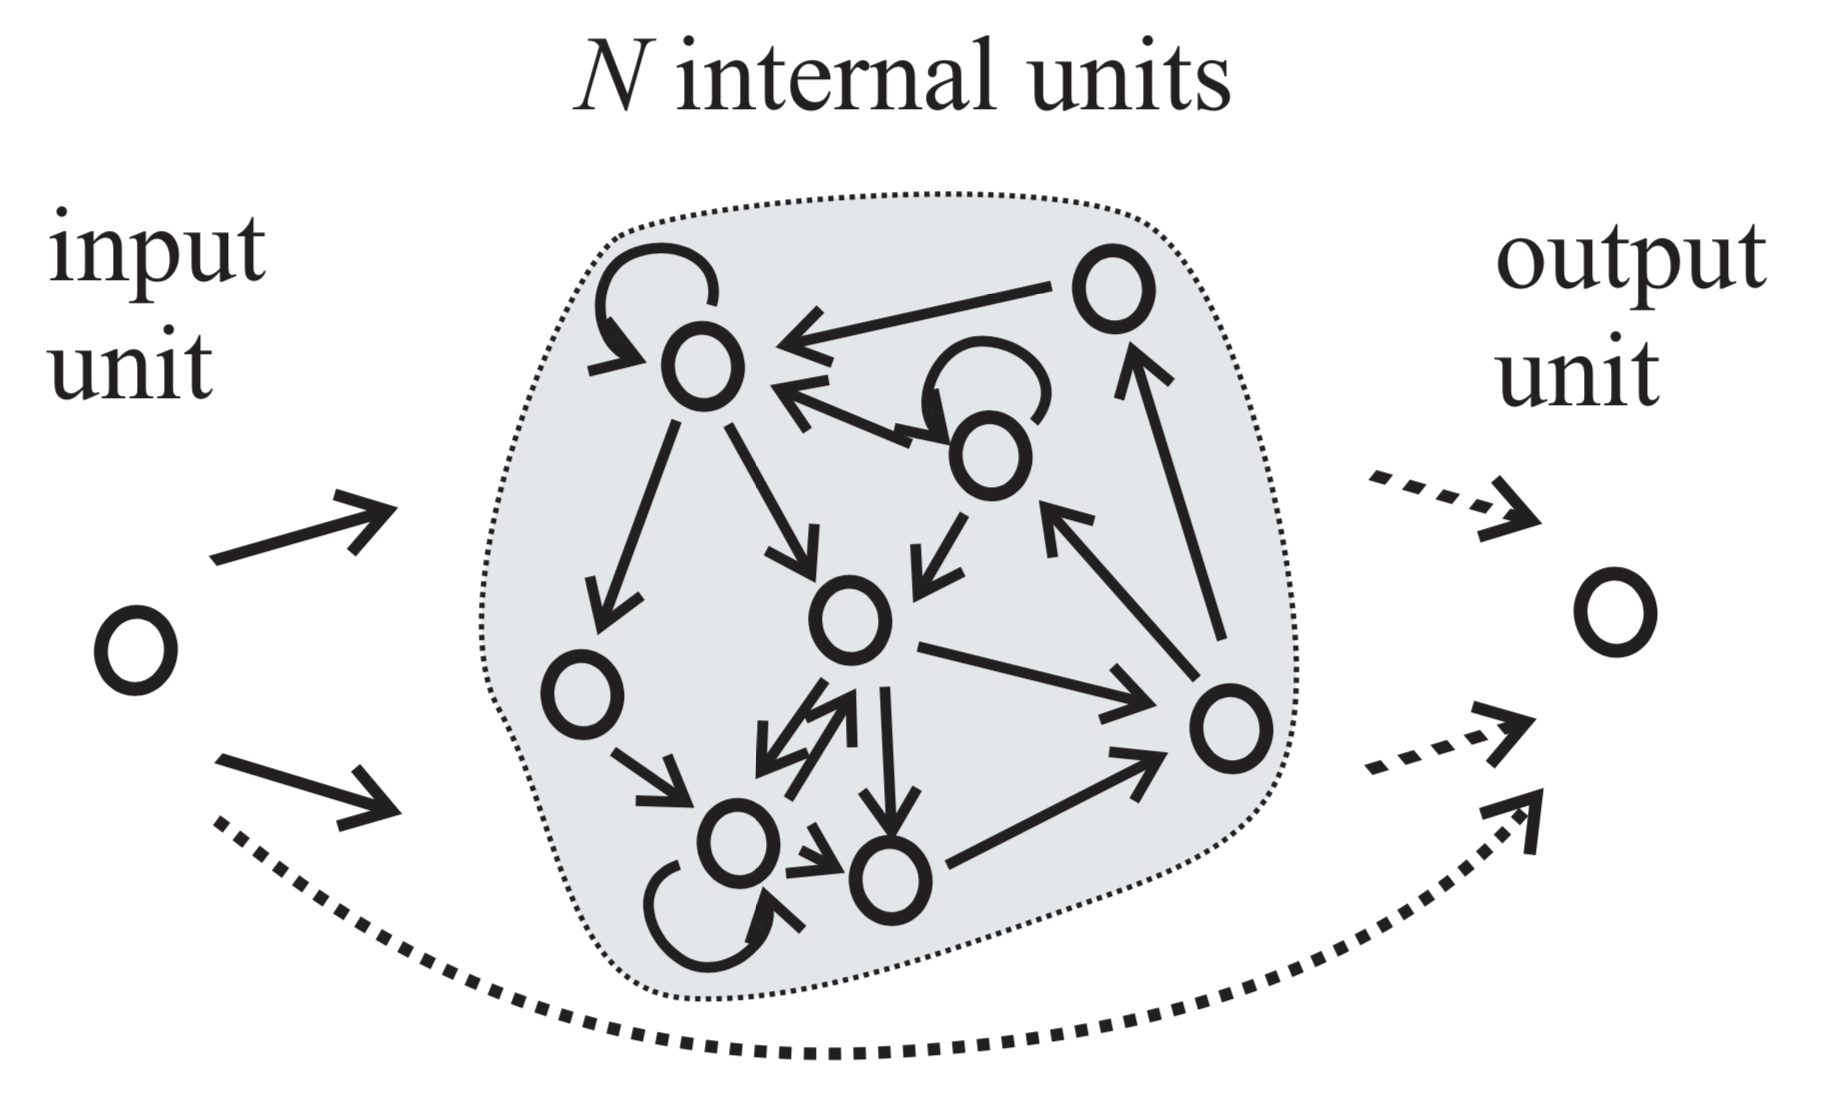
\includegraphics[width=0.7\textwidth]{Pictures/BasicESNStructure.png}
    \end{center}
    \label{FIG:ESNArchitecture}
    \caption{The basic structure of an ESN. Figure taken from \cite{Jaeger2003}. Dotted lines represent trainable connections, whereas solid arrows are fixed connections.}
\end{figure}

Most of the time, the network is being adapted to a specific time series and is trained to perform 1-step ahead predictions, so $u = By$\footnote{B is the backshift operator is defined as $B: \left(\R^n\right)^{\Z} \to \left(\R^n\right)^{\Z}$, $\left(z_t\right)_{t\in\Z} \mapsto \left(z_{t-1}\right)_{t\in\Z}$.}.

Other versions of the basic model can include feedback connections from the output back to the reservoir or the application of leaky-integrator neurons \citep{JAEGER2007335}.
For $\alpha \in \left[0, 1\right]$ and $\wfb \in \R^{N\times L}$ the dynamics of the system \refp{EQ:ReservoirUpdate} accordingly change to
\begin{eqnarray}
    \tilde \bx_t & = & W\bx_{t-1} + \win u_t +  \bb + \wfb y_{t-1} \label{EQ:UpdateLeakyIntegrator}\\
    \bx_t & = & f\left(\alpha \bx_{t-1} + (1-\alpha) \tilde \bx_t \right) \\
    y_t & = & \bx_t \wout  \label{EQ:ESNOutput}
\end{eqnarray}
The leak parameter $\alpha$ can be interpreted as a parametrical way of keeping information within the reservoir nodes. For example, a value of $\alpha = 0.2$ would make the neuron keep $20\%$ of its current information and only allow the newly arriving value of $\tilde x(t)$ to complement this value with a weight of $80\%$. Leaky-integrator neurons would theoretically be possible for the remainder of this thesis but have not been used.

Feedback connections pose a challenge to the training of an Echo State Network because the output connections $\wout$ have to be solved iteratively (because of the need for an output value $y_{t-1}$ in the update \ref{EQ:UpdateLeakyIntegrator}). This could be achieved by an online learning approach (see section \ref{CH:LinearRegression:Online}). However, if the input is chosen as $u = By$ to produce one-step-ahead forecasts of $y$, the target output $y_t$ is the new input to the network by design.

\subsection{Training}

In order to map the network state to a desired output, $\wout$ in \refp{EQ:ESNOutput} can be trained using a linear regression model from section \ref{CH:LinearRegression}.
Hence, the network is being fed the input signal and activations $x_t$ are gathered in a matrix $\tilde X = \left[\bx_0'; \bx_1'; ...; \bx_T'\right] \in \R^{T\times N}$. This regressor matrix can be further enhanced by the addition of an intercept or by the the network input $u$ so that $X = \left(1_{N}, u, \tilde X\right) \in \R^{T\times(2+N)}$.
One could also employ more sophisticated (machine learning) models to map the network activations and the desired output. However, the Echo State Network convinces by its simple and fast training. Additionally, the theory of (high dimensional) linear regression has been studied extensively.

In the training of $\wout$ one has to keep in mind, that the network state has been initialized with $\bx_0 = {\bf 0} \in \R^{N}$. To wash out the effect of the initial state and to prevent misleading training results, an initial transient $\tau$ of observations has to be dropped. The echo state property which will be introduced in section \ref{CH:ESN:ESP} will guarantee, that the effect of (any) initialization fades after several updates of the network. 
This transient can be chosen as a fixed number, or - depending on the size of the dataset - can be set to a fraction of the whole dataset, i.e. $\tau = 0.05\cdot T$. The regressor matrix is truncated accordingly.


\subsection{Hyperparameters}
\label{CH:ESN:Hyperparameters}

Training of Echo State Networks is simple and fast. Most of the connections within the network are initialized randomly and will not be trained to adapt the system to a given task. However, the initialization of those connections has  - as almost all machine learning models do - some hyperparameters that need to be chosen in advance. The choice of (some of) these parameters plays a crucial role in the performance of the model and therefore need special attention. Analytic derivations of optimal parameters are very difficult because of the dynamic and iterative nature of the reservoir. For some there is no analytical solution and other methods such as basic grid search, particle swarm optimization \citep{basterrech2015experimental} or gradient descent \citep{JAEGER2007335} have to be employed. This weighs heavily on the training of time of Echo State Networks. On the other hand, this is also the case for other machine learning models. In the following, we want to present the hyperparameters that are specific to Echo State Networks and come as a tradeoff for not having to train internal connections. % TODO February 29, 2020 : add more
We will go into more detail on the methodology of choosing hyperparameters in section \ref{CH:Application:Methodology}.


\subsubsection{Underyling Probability Distribution of Connections}

In order to initialize the fixed connections within the dynamical system (i.e. $\win$, $W$, $b$), one has to choose some probability distribution\footnote{Typically, the same distribution is chosen for all random initializations.}. Typical choices include the discrete bi-valued\footnote{The discrete bi-valued distribution of weights has a positive chance of creating identical neurons but makes analysis of the reservoir dynamics much easier.} $\mathcal{U}\left\{-1, 1\right\}$, the uniform $\mathcal{U}(-1, 1)$ or the normal distribution $\mathcal{N}(0, \sigma^2)$ for some $\sigma >0$. Even though, \cite{Wu2018StatChallenges} show that the choice of the distribution has an effect on performance, the probability distribution as a hyperparameter doesn't receive much attention and researchers rarely shed any light on their specific choice. Other sources state, that different distributions give almost the same performance because the other hyperparameters are of much higher importance \citep{Lukosecicius2012}. After all, it is worth noting that the distribution of internal weights bears some freedom of choice and may possibly be worth exploring for some tasks.

\subsubsection{Sparsity}

Sparsity is referring to the number of non-zero elements in the internal connections $W$. \cite{Jaeger2004Harness} use a 1\% connectivity to establish a richly structured reservoir of excitable dynamics. Apart from the richness of the reservoir, the computational cost of updating the reservoir is significantly reduced when the connectivity is chosen in relation to the number of total connections. By choosing the sparsity as a fraction of total connections by $s = 10/N^2$ the cost of updating the network only grows linearly with the size of the reservoir instead of quadratically.

\subsubsection{Spectral Radius}

The spectral radius of the internal connections $W$ is the most important hyperparameter for the Echo State Network as it is mainly responsible for the echo state property and the memory capacity of the reservoir. The larger the spectral radius, the more dominant is the echo state (the first part of the update \ref{EQ:ReservoirUpdate}) of the reservoir compared to the new input. So a higher spectral radius means that the reservoir has longer memory and a smaller spectral radius renders the reservoir predominantly a respresentation of the most recent input \citep{Lukosecicius2012}. Depending on the task at hand, one can use some intuituion on the range of plausible spectral radii.


\subsection{Echo State Property}
\label{CH:ESN:ESP}

The echo state property (ESP) is a necessary condition for the network to be able to produce exploitable patterns. Loosely speaking, the echo state property states that the network state is asymptotically independent of its initial state \citep{Jaeger2003}. In other words, the network will forget its initial state and will only depend on a finite set of inputs $u_t$ from a compact set and will forget its initialization, typically ${\bf 0} \in R^{N}$.
The literature offers different approaches to ensure the echo state property. Orginially, \cite{Jaeger2001} stated that choosing the internal connections $W$ such that the spectral radius $\rho(W) = \max \left\{\lambda \,:\, \lambda \text{ eigenvalue of} W\right\}$ is less than unity, would ensure the echo state property for all inputs $u$. This lead to a widespread misconception that the spectral radius always \textit{has} to be smaller than unity. However, depending on the input, larger spectral radii can also be possible without counteracting the echo state property \citep{YILDIZ20121}. \cite{YILDIZ20121} also propose to look at the spectral radius of the corresponding positive matrix $\rho(\abs{W})$ and to ensure that its spectral radius is less than unity. \cite{Ozturk2007AnalysisDesign} propose a procedure to maximize the average state entropy by a spectrum of eigenvalues in the complex plane. \cite{Strauss2012Design} state that the echo state property should be based on the singular values of the connections $W$ instead of its spectral radius. They propose to choose the singular values to be smaller than $1$ to ensure the echo state property. Additionally, the activation function has to be Lipschitz continuous with constant 1\footnote{Which is the case for $tanh$.}. They obtain a sparse and orthogonal matrix $W$ whose singular values and eigenvalues are known to ensure the echo state property.
As there is now direct way to ensure the echo state property for a given input sequence, and some of the above restrictions limiting the performance of the network, the choice of hyperparameters and ensuring for the echo state property falls back to a try-and-error methodology. It is desirable to bring the network dynamics towards the \textit{edge of chaos}, which means to push the dynamics close towards the border between a stable and an unstable regime \citep{LengensteinMaass2007EdgeOfChaos, Buesing2010} to improve computational outcome. 

The choice of the hyperparameters, especially the spectral radius, motivates the following section which targets the tuning of the reservoir beyond its random initialization.


\subsection{Tuning of the Reservoir Dynamics}
\label{CH:ESN:Tuning}

The motivation for the inclusion of this section stems from the nature of another reservoir computing model, namely the State Affine Systems \citep{Grigortega2018SAS}, which changes its dynamics given newly presented input. An Echo State Network is indeed dynamical system, however, the connections within the network are fixed and don't change. They can be interpreted as a restricted and slightly modified State Affine System, where its dynamics, namely $W$ or $\win$, are functions of the input.
This motivated the search for ways to modify the Echo State Network to react differently to different inputs, adapt its dynamics or in general to further improve the reservoir after initialization.

Different endeavours have been undertaken to tune the reservoir beyond the random initialization and the selection of hyperparameters. As mentioned earlier, the most import hyperparameter is the spectral radius\footnote{Other hyperparameters are important as well, but the spectral radius has the largest effect on the performance of the network.}.
\cite{Triesch2005} uses an unsupervised intrinsic learning approach to change the neurons excitability beyond the its random intialization. Using a continuous activation model, he tries to bring the output of each neuron as close as possible to an exponential distribution. 

In order to tune the neuron's output, he transforms the original activation function $f: \R \to \R$, $\bx \mapsto \frac{1}{1+\exp{-\bx}}$ (fermi activation function) using
\begin{equation}
    f_{y}(y) = f(\balpha\odot \bx + \bbeta)
\end{equation}
with tunable parameters $\balpha, \bbeta  \in \R^{N}$. To match the notation of \cite{Triesch2005} and \cite{Schrauwen2008}, $y$ in this instance is not be confused with the network output but represents the post-activation network state. We use vector notations for $\bx, \balpha$ and $\bbeta$ as each element of $\balpha$ and $\bbeta$ is related to a neuron in the network. The modified network update not only tunes the spectral radius but also incorporates the bias $\bb$. The effective update of the network then becomes
\begin{equation}
    \bx_t = f\left(\diag{\balpha}W\bx_{t-1} + \diag{\balpha}\win u_t + \balpha \odot \bb + \bbeta\right)
\end{equation}

Using a gradient descent method, he minimizes the Kullback-Leibler divergence of the transformed output $y$ and the desired output distribution. 
\begin{eqnarray}
    D_{KL} \left(f_y \,\vert\vert\, f_{exp}\right) & = & \int f_y(y) \, \log{\frac{f_y(y)}{\frac{1}{\mu} \exp{\frac{-y}{\mu}}}} \dd y\\
    & = & \int f_y(y) \, \log{f_y(y)} \dd y - \int f_y(y) \, \left(-\frac{y}{\mu} - \log{\mu}\right) \dd y \\
    & = & -H(y) + \frac{1}{\mu} \E{y} +  \log{\mu}
\end{eqnarray}
Where $H(y)$ is the entropy of $y$, and $\E{\cdot}$ is the expectation. In other words, he tries to make the output $y$ be as close as possible to $\frac{1}{\mu} \exp{-y/\mu}$. The last term $\log{\mu}$ is constant and the second term $\frac{1}{\mu}\E{y}$ is equal to $1$ if $y$ follows an exponential distribution with parameter $\mu$. This shows, that the exponential distribution is the maximum entropy distribution \citep{Triesch2005}. Therefore the Kullback-Leibler divergence is minimized, when the entropy is maximized\footnote{This implies the direct connection of the fermi activation function and the exponential distribution.}. Using the gradient with respect to $\balpha$ and $\bbeta$, he comes up with the following stochastic gradient descent rule for $\balpha := \balpha + \Delta\balpha$ and $\bbeta := \bbeta + \Delta\bbeta$ with
\begin{eqnarray}
    \Delta\bbeta & = & \eta \left(1 - \left(2+ \frac{1}{\mu}\right)y + \frac{1}{\mu}y^2 \right) \\
    \Delta\balpha & = & \eta \left(\frac{1}{\balpha} + x - \left(2+ \frac{1}{\mu}\right)\bx y + \frac{1}{\mu}\bx y^2\right) \\
    & = & \frac{\eta}{\balpha} + \Delta\bbeta x
\end{eqnarray}
where $0 < \eta < 1$ is a small learning rate. % TODO February 29, 2020 : much less sign


Different extensions of \cite{Triesch2005} have been proposed, including \cite{Boedecker2009SelfOrganized} who match the neurons' output to a Laplace distribution. Another extension is provided by \cite{Schrauwen2008} who target a gaussian output distribution $\mathcal{N}\left(\mu, \sigma^2\right)$ using the hyperbolic tangent as activation function which is the maximum entropy with support $\left[-\infty, \infty\right]$. They follow the argumentation along the lines of \cite{Triesch2005} and come up with similar updates of the parameters $\balpha$ and $\bbeta$, namely\footnote{They use an equivalent notation for \refp{SchrauwenUpdate1}: $\Delta\beta = - \eta \left(-\frac{\mu}{\sigma^2} + \frac{\by}{\sigma^2}\left(2\sigma^2 + 1 - \by^2 + \mu \by\right)\right)$.}:

\begin{eqnarray}
    \Delta \bbeta & = & -\eta \left(2y + \frac{1}{\sigma^2} \left(1 - y^2\right)\odot(y-\mu)\right) \label{SchrauwenUpdate1}\\
    \Delta \balpha & = & \frac{\eta}{\balpha} + \Delta\bbeta \odot \bx \label{SchrauwenUpdate2}
\end{eqnarray}

\citep{Schrauwen2008} recognize, that the boundedness of the activation function influences the output distribution of the neurons and in turn imposes a certain constraint on the moments of the infinite normal distribution. They analyse the behaviour of their online update and the resulting empirical distributions and find that for certain choices of $\mu$ and $\sigma$ the boundedness significantly truncates the distribution. However, this problem can be easily solved by introducing another transformation of the activation function which is one of the contributions of this thesis. Given $c > 0$ we transform the activation function
\begin{equation}
    f_y(y) = c \cdot \tanh{\frac{\balpha \odot \bx + \bbeta}{c}}
\end{equation}
such that the activation functions maps to the interval $[-c, c]$. Choosing $c$ depending on the parameters of the normal distribution, i.e. the $99.5\%$ quantile or any arbitrary value larger than that, the probability mass that is being truncated by the activation function can be chosen arbitrarily small. The online learning rule for $\alpha$ and $\beta$ straightforwardly becomes:
\begin{eqnarray}
    \Delta \bbeta & = & -\eta \left( \frac{2y}{c^2} + \frac{1}{\sigma^2} \left(1 - \frac{\by^2}{c^2}\right)(\by-\mu)\right) \\
    \Delta \balpha & = & \frac{\eta}{\alpha} + \Delta \beta \bx
\end{eqnarray}
which is equivalent to \refp{SchrauwenUpdate1}-\refp{SchrauwenUpdate2} for $c = 1$. This enables us to choose any value of $\sigma > 0$\footnote{Other activation functions like the $arcsinh$ \citep{KIM2001ARCSINHActivation} or a rectified natural logarithm \citep{Liu2019NaturalLogarithmRectifiedAF} have been considered to achieve the goal of variable boundedness of the activation function but given the solution presented above, have not been further explored.}. The choice of $\mu$ is still limited but can be neglected. This is because network activations centered around $0$ or centered around $\mu \neq 0$ provide the same information and the linear readout can take care of any necessary shift. Figure \ref{FIG:IPTuning} presents the effect of the adaptation of the reservoir towards a target output distribution. The fit is clearly improved and the introduction of the scaling parameter $c$ is justified as we find activation values outside $\left[-1, 1\right]$.


\begin{figure}
    \begin{center}
    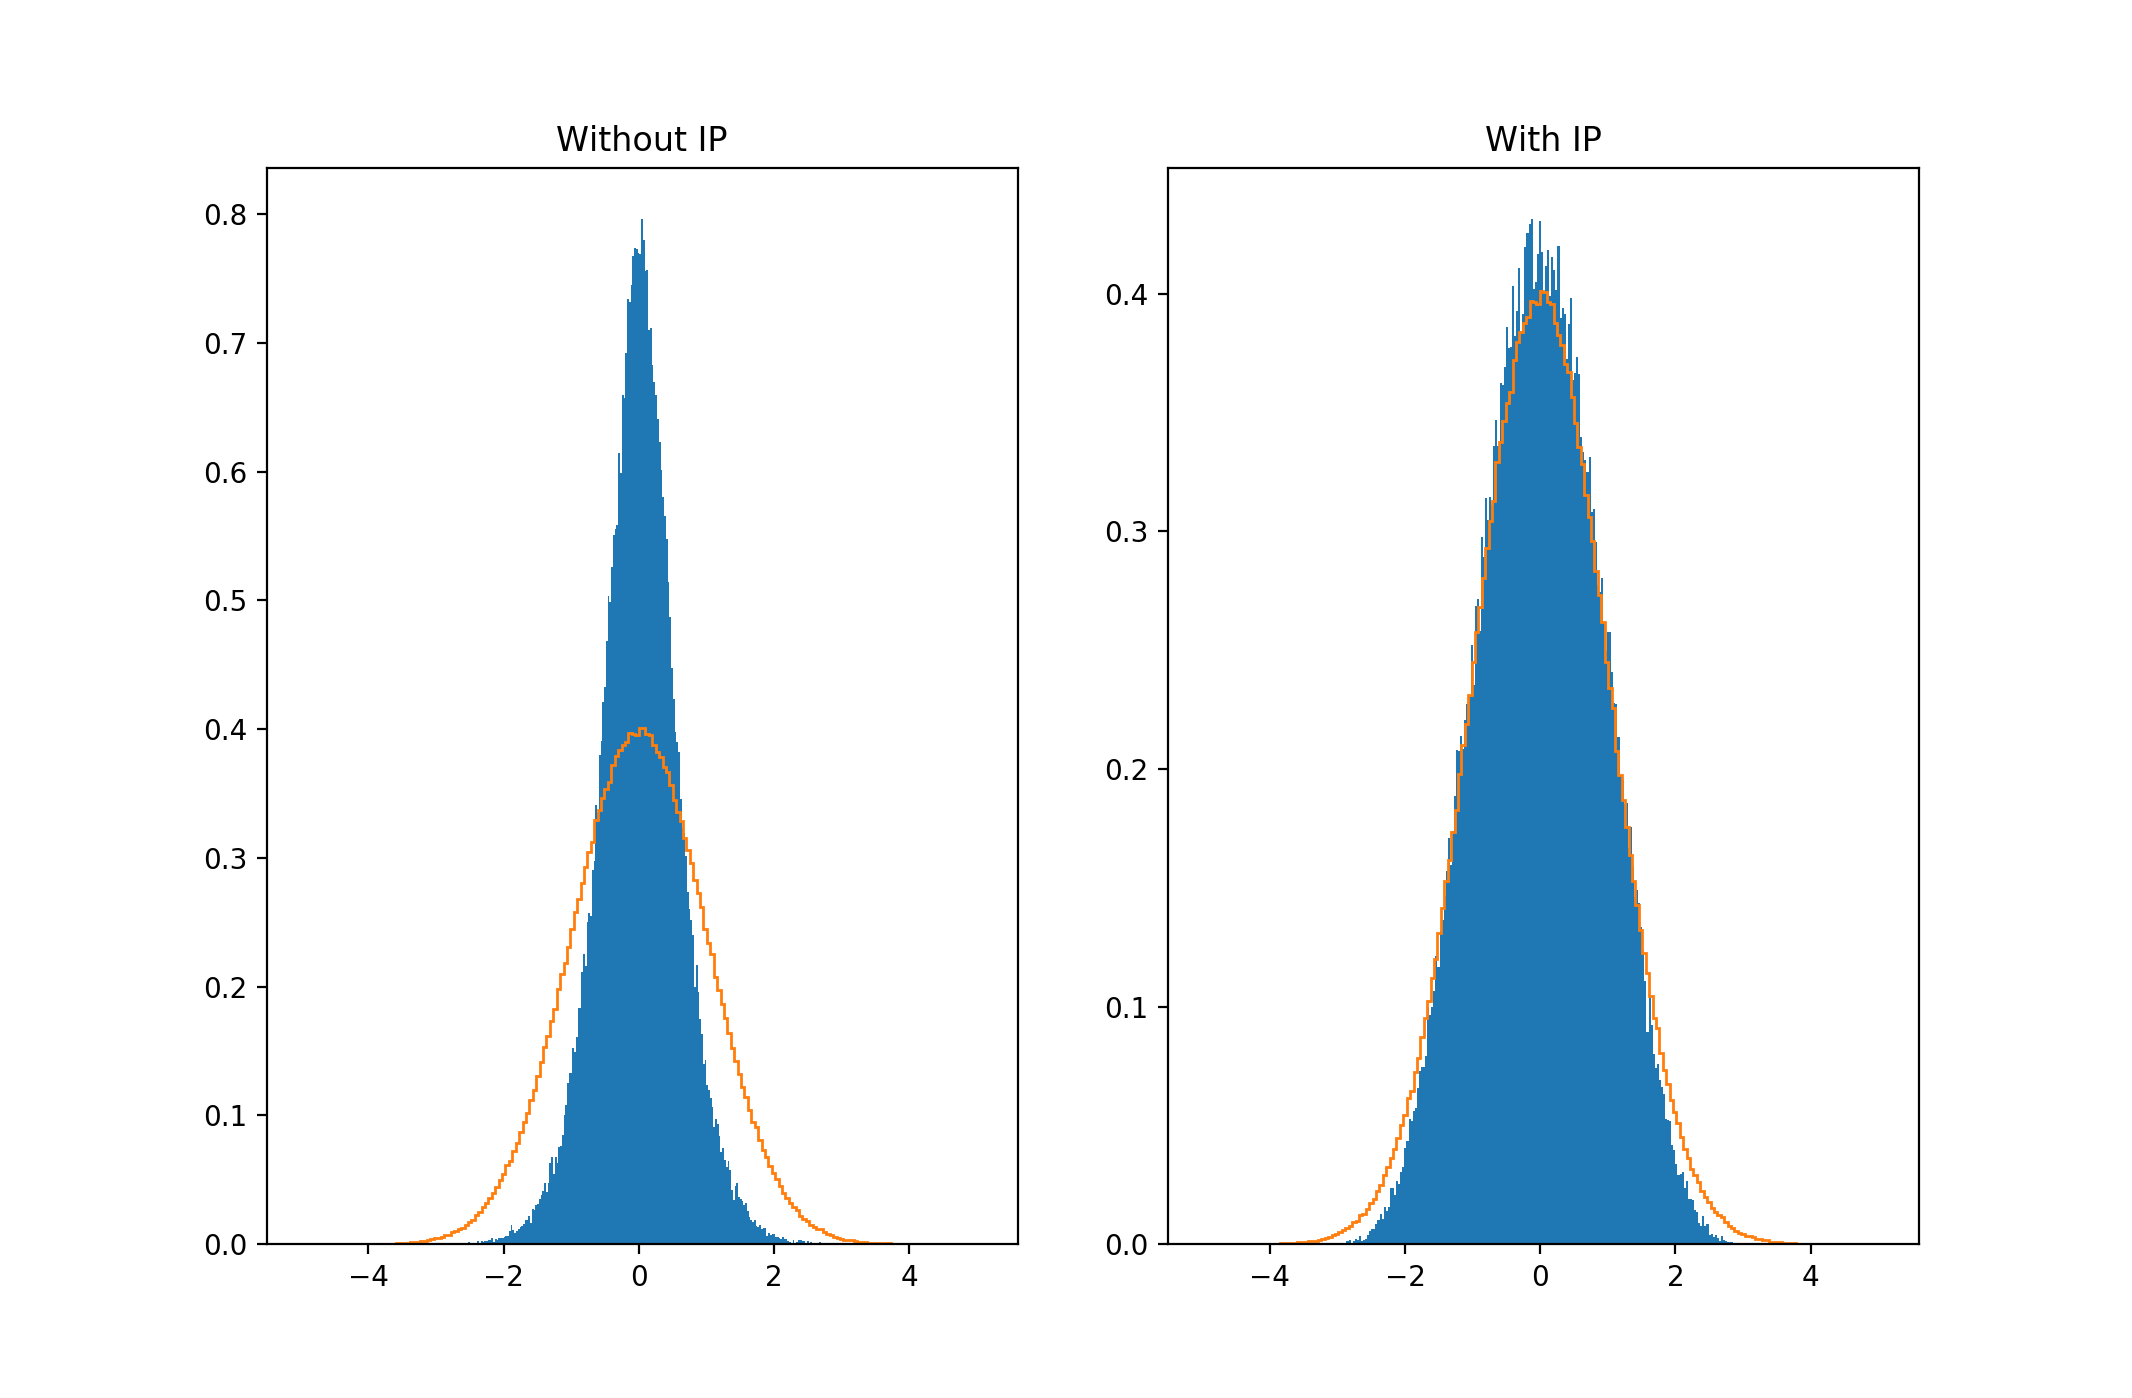
\includegraphics[width=0.9\textwidth]{Plots/IP_KLTANH_sigma1.png}
    \end{center}
    \label{FIG:IPTuning}
    \caption{Network activations of a standard Echo State Network of size $N=1000$ with initial spectral radius of $\rho = 0.95$. Its activation function, as can be seen by the range of activation values, has been adjusted to allow for a wider range of values. The fit of the last $100$ network activations is clearly improved by the transformation. Additionally, the activation values are larger than $1$ which supports the additional of the scaling parameter $c$. Adaptation of the reservoir has been performed for $100$ epochs feeding the Mackey-Glass timeseries of length $5000$ and the scaling of the activation function was chosen as $c=5$.}
\end{figure}

Furthermore, \cite{Koprinkova2011IPandStability} show that the pre-training of an Echo State Network using intrinsic plasticity improves the network stability. They find a close relationship between IP pre-training and stabilization of the reservoir dynamics, such that even initially unstable reservoirs become stable by pushing reservoir activations towards the predefined mean $\mu$ of the normal distribution. They derive the Kullback-Leibler divergence as
\begin{equation}
    D_{KL} = - H(y) + \frac{1}{2\sigma^2}\E{\left(y-\mu\right)^2} + \log{\frac{1}{\sigma\sqrt{2\pi}}}
\end{equation}
which shows the compromise between entropy maximization and minimization of the distance between $\mu$ (typically chosen as $0$) and $y$.